%%
%% Copyright 2024 OXFORD UNIVERSITY PRESS
%%
%% This file is part of the 'mam-authoring-template Bundle'.
%% ---------------------------------------------
%%
%% It may be distributed under the conditions of the LaTeX Project Public
%% License, either version 1.2 of this license or (at your option) any
%% later version.  The latest version of this license is in
%%    http://www.latex-project.org/lppl.txt
%% and version 1.2 or later is part of all distributions of LaTeX
%% version 1999/12/01 or later.
%%
%% The list of all files belonging to the 'mam-authoring-template Bundle' is
%% given in the file `manifest.txt'.
%%
%% Template article for Microscopy and Microanalysis' document class `mam-authoring-template'
%% with bibliographic references
%%

\documentclass[unnumsec,webpdf,modern,large]{mam-authoring-template}%
	
%\usepackage{showframe}

\graphicspath{{Images/}}

% line numbers
%\usepackage[mathlines, switch]{lineno}
%\usepackage[right]{lineno}

\theoremstyle{thmstyleone}%
\newtheorem{theorem}{Theorem}%  meant for continuous numbers
%%\newtheorem{theorem}{Theorem}[section]% meant for sectionwise numbers
%% optional argument [theorem] produces theorem numbering sequence instead of independent numbers for Proposition
\newtheorem{proposition}[theorem]{Proposition}%
%%\newtheorem{proposition}{Proposition}% to get separate numbers for theorem and proposition etc.
\theoremstyle{thmstyletwo}%
\newtheorem{example}{Example}%
\newtheorem{remark}{Remark}%
\theoremstyle{thmstylethree}%
\newtheorem{definition}{Definition}
\usepackage{tikz}
\usepackage{physics}
\usepackage{bm}
\usepackage{pgfplots}
\pgfplotsset{compat=1.15}
\usepackage{mathrsfs}
\usepackage{xcolor}
\usepackage{graphicx}
\usepackage{caption}
\usepackage{subfigure}
\usepackage{subcaption}
\usetikzlibrary{arrows}
\usepgfplotslibrary{fillbetween}
\pgfmathdeclarefunction{gauss}{2}{%
	\pgfmathparse{1*exp(-((x-#1)^2)/(2*#2^2))}%
}

\begin{document}
	\journaltitle{Selected Topic In Physics}
	%\DOI{DOI HERE}
	\copyrightyear{2024}
	\pubyear{2024}
	%\access{Advance Access Publication Date: Day Month Year}
	\appnotes{Original Article}
	
	\firstpage{1}
	
	%\subtitle{Subject Section}
	
	\title[Overview On Quantum Hall Effect]{Overview On Quantum Hall Effect}
	
	\author[1,$\ast$]{Vo Chau Duc Phuong\ORCID{0000-0003-0978-916X}}
	
	\authormark{Vo Chau Duc Phuong}
	
	\address[1]{\orgdiv{Condensed Matter and Statistical Physics}, \orgname{ICTP},\orgaddress{ \country{Italy}}}
	
	\corresp[$\ast$]{Corresponding author. \href{email:vcdphuong@outlook.com}{vcdphuong@outlook.com}}
	
%	\received{Date}{0}{Year}
%	\revised{Date}{0}{Year}
%	\accepted{Date}{0}{Year}
	
	\abstract{about one line on the link between the classical and quantum hall effect. Some line on the effect of QHE on or from the topology or Berry phase of material}
	\keywords{Overview, quantum Hall effect}
	
	% \boxedtext{
		% \begin{itemize}
			% \item Key boxed text here.
			% \item Key boxed text here.
			% \item Key boxed text here.
			% \end{itemize}}
	
	\maketitle
	

	
\section{Introduction}\label{Intro}


\subsection{From classical Hall effect}\label{Introsub1}
\quad The Hall effect happens when a conductor with a flow of current being placed in an external magnetic field \(\textbf{B}\). The Lorentz force of the magnetic field make the charge move to one side of the conductor. The equilibrium will be established when the charge density of both side create a strong enough electrical field \(\textbf{E}\). The relation between the current density and electric field can be described by Ohm's law (see Appendix \ref{particle in field}):
\begin{equation}\label{Ohm}
	\textbf{J} = \sigma \textbf{E} \quad \rightleftharpoons \quad \textbf{E} = \rho \textbf{J},
\end{equation}
where the conductivity \(\sigma\), in principle, is a second rank tensor, showing the affect on a direction from electric field of another direction. In the absent of the magnetic field or in the anisotropy materials, the off-diagonal element can be considering to be 0 without any further concern. In that case, the Ohm's law read:
\begin{equation}\label{Ohm diag}
	\textbf{J} = \bigg(\frac{n_e e^2 \tau_L}{m_e}\bigg) \textbf{E},
\end{equation} 
in which, \(n_e, e,\tau_L,\) and \(m_e\) is density of electron, element charge, relaxation time (from scattering), and mass of electron, respectively.\\
\null\quad Placing this system an external uniform magnetic field \(\textbf{B} = (0,0,B)\) and using the convention of choosing x-axis parallel to the current direction. In this convention, Ohm's law reads:
\begin{equation*}
	\begin{pmatrix}
		E_x\\E_y
	\end{pmatrix}
	= \begin{pmatrix}
		\rho_{xx} & \rho_{xy}\\
		-\rho_{xy} & \rho_{yy}
	\end{pmatrix}
		\begin{pmatrix}
		J_x\\J_y
	\end{pmatrix}.
\end{equation*}
\quad The \textit{resistivity} \((\rho)_{ij}\) define as the inverse of the \textit{conductivity} \((\sigma)_{ij}\). From Drude model, we have explicitly:
\begin{equation}
	\rho
	=\frac{1}{\sigma_{DC}} \begin{pmatrix}
		1 & \omega_B \tau\\
		-\omega_B \tau & 1
	\end{pmatrix}
\end{equation}
The off diagonal element
$$\rho_{xy} = \frac{\omega_B \tau}{\sigma_{DC}}$$
independence of the scattering time \(\tau\). Measuring the ratio between the \(V_y\) and current \(I_x\)
\begin{equation}
	R_{xy} = \frac{V_y}{I_x} = \frac{E_y L}{J_x L} = \frac{E_y}{J_x},
\end{equation}
for so called \textit{the resistance} R. Equation above correspond to,
\begin{equation}
	R_{xy} =  \frac{E_y}{J_x} = -\rho_{xy} = - \frac{\omega_B \tau}{\sigma_{DC}}.
\end{equation}
\quad Defining the Hall resistance as
\begin{equation}\label{Hall def.}
	R_H = -\frac{R_{xy}}{B} = \frac{\rho_{xy}}{B} = \frac{1}{n e},
\end{equation}
\quad showing that the Hall resistance is a constant in the classical regime.\\
So far, we show that the classical resistance tensor have the form of depend on either the scattering time \(\tau\) or the magnetic field \(B\):
\begin{equation}
	\rho = \begin{pmatrix}
		\frac{m}{ne^2\tau} & \frac{B}{ne}\\
	- \frac{B}{ne} & \frac{m}{ne^2\tau}
	\end{pmatrix}
\end{equation}
\subsection{To the discover of the quantum Hall effect}\label{Introsub2}
\quad Thing changes when we cooling down the system to extreme and increase the magnetic field \((\sim 1 T)\). As shown in (ref{Kitzling 1980}), at certain gate voltages, the conductivity go to 0 even when the density of carrier increase ref(Ando 1971) (corresponding to the strength and the concentration of the scatterer in the article). Further investigation showing that due to the governing of the quantum mechanics, there are two separate phenomenons, called \textit{integer} and \textit{fractional} quantum Hall effect. Hereby then, we will overview the basic concepts of these two effects and leave the more theoretically part in another section (see section \ref{Integer QHE theory} and section \ref{Fractional QHE theory}).
\subsubsection{Integer quantum Hall effect} \label{Integer QHE Overview}
\quad From the precisely measurement of ref{Kitzling 1980}, which will brought him a Nobel award in 1980, as can be seen in figure (include Kitzling figure and integer qunatum hall effect figure). The \textit{longitude} and \textit{transverse resistance} showing a very interesting properties in the low temperature and high magnetic field.\\\null
\quad The \textit{longitude resistance} \(\rho_{xx}\) go to 0 at certain gate voltages (\(B\) fixed in the figure ref figure kitzling) et vice verse (vary the field \(B\) while keep other parameters), showing that there's none resist for the current, or in another words: Superconducting.\\ \null
\quad Even more interesting is the Hall resistance, or \textit{transverse resistance} \(\rho_{xy}\). It jumps from plateau to plateau, significantly showing the quantization properties. In section \ref{Integer QHE theory}, It will be shown to be obey\footnote{A little remind: the non-zero integer \(\mathbb{Z} \backslash \{0\}\) has been used instead of the \(\mathbb{N}^*\) for the skew symmetry of \(\rho\)}
\begin{equation}\label{off diag rho}
	\rho_{xy} = \frac{2\pi \hbar}{e^2} \frac{1}{\nu} \quad \nu \in \mathbb{Z} \backslash \{0\}
\end{equation}
\quad This properties shows that through measuring the Hall resistance, not only evaluate directly the Kitzling constant \(2\pi \hbar/e^2\) but also a well-known \textit{fine structure constant} \(\alpha\).
\subsubsection{Fractional quantum Hall effect} \label{Fractional QHE overview}
\quad Recently, we just discussed the results on the nearly pure samples. This "impurity" has another name is \textit{disorder}. Interestingly, as we decrease the \textit{disorder} of the sample, i.e. made it purer, better, the plateau in the data disappear, which will be covered in ref{Interger QHE}.\\\null
\quad As we increase the disorder even more, the integer peaks and plateaus become less prominent. Instead of that, according to ref{Tsui 1982} data, there are other plateaus obey the same relation shows in \eqref{off diag rho}, however with \(\nu\) as a fractional number:
$$\nu \in \mathbb{Q}.$$
\quad Not all fractions appear, some are proof to be more prominent than the others.\\\null
\quad In general, while the integer quantum Hall effect can be explained by the free electron model, the interactions between the electrons have to be taken into accounted to explain the fractional quantum Hall effect.
\section{Materials}
\quad It is worth to have some lines about the materials, in which we found and observed both the integer and fractional effects.The integer effect has been observed first time in \(Si\) MOSFET ref{Kitzling 1980} and then later on in \(GaAs-GaAsAl\) heterostructure\footnote{both of these material have density of electron \(n \sim 10^{11} - 10^{12} cm^{-2}\)}. More recently works also show these effect in Gaphene and other materials. Sometimes, the appear of quantum Hall effect in two material can be the same in spirit but differ in details.
%This effect happens due to Landau level (see appendix )when a 2D free electron placed in a magnetic field.\\\null
%\quad Without the field, the density of states (DOS) have the form of 2-D free electron gas, independence with the energy,
%\begin{equation}\label{DOS fermi 2D}
%	n_{2D} = \frac{m^*}{\pi \hbar}.
%\end{equation}
%\quad When turning on the field at 0K, the DOS collapse from the constant \ref{DOS fermi 2D} to the Dirac comb (a set of Dirac function at certain energy states). At finite temperature, DOS spread about the Landau energy due to the scattering({\color{red} include figure about Landau level and spreading}). If the spacing between levels bigger than the scattering, we will have the distinct spectrum.

\section{The Integer Quantum Hall effect}\label{Integer QHE theory}
\subsection{Long Story Short}
\quad According to the data of experiments, we have the Hall's resistance in compare with the Drude model:
\begin{equation}
	\rho_{xy} = \frac{2\pi \hbar}{e^2 \nu} = \frac{B}{n e}.
\end{equation}
\quad Giving us the density of charge need to reach the resistivity corresponding with number \(\nu\):
\begin{equation}
	n = \frac{eB}{2\pi \hbar}\nu= \frac{B}{\Phi_0}\nu,
\end{equation}
where
\begin{equation}\label{def Phi_0}
	\Phi_0 =\frac{2\pi \hbar}{e}= \frac{h}{e}.
\end{equation}
\quad Considering when the system completely fill the \(\nu\)-th Landau level, there's no where for the electron to run inside that Landau's state. The electrons stay in the same place, cause no scattering, which also mean \(\tau \to \infty \Rightarrow \rho_{xx} \to 0\) as the data show\footnote{These condition happen due to our assumption that the thermal energy \(k_B T\) very small in compare with the gap caused by Landau levels.}.\\\null
%\subsection{Conductivity in Quantum Mechanics}
\quad A particle inside the electromagnetic field according to Ehrenfest's theorem have the velocity
\begin{align}
	i\hbar\dot{\textbf{x}} &= \comm{\textbf{x}}{\frac{(\textbf{p}-e\textbf{A})^2}{2m}} = \comm{\textbf{x}}{\frac{\textbf{p}^2 -2 eA\textbf{p}+(eA)^2}{2m}}\nonumber\\
	&= \frac{1}{2m}\comm{\textbf{x}}{\textbf{p}.\textbf{p}} -  \frac{1}{2m} 2e\textbf{A} \comm{\textbf{x}}{\textbf{p}}\nonumber\\
	\Rightarrow m\dot{\textbf{x}}&= \textbf{p} -e\textbf{A}
\end{align}
The total current of the system is:
\begin{align}
	I &= -e\ev{\dot{\textbf{x}}} = -\frac{e}{m} \sum_{\text{filled}} \ev*{\textbf{p} -e\textbf{A}}{\psi}\\
	&= -\frac{e}{m} \sum_{n} \sum_{k_y}  \ev*{\textbf{p} -e\textbf{A}}{\psi_{n,k}(x)}
\end{align}
If we chose the Landau gauge convention: \(\textbf{A}= (0,xB,0)\), and place electric field \(\textbf{E}\) along the \(O_x\), along the x direction, we have:
\begin{equation}
	I_x = -\frac{e}{m} \sum_{k_y} \sum_{n =1}^\nu \ev*{\frac{\hbar}{i} \partial_x}{\psi_{n,k}(x)},
\end{equation}
this one vanishes due to the orthogonal properties of the Hermitian function. Meanwhile, along the other direction:
\begin{align}
	I_y &= -\frac{e}{m}\sum_{n}^\nu\sum_{k_y} \ev*{\frac{\hbar}{i}\partial_{y} - eBx}{\psi_{n,k_y}(x)}\nonumber\\
	\label{Iy}
	&= -\frac{e}{m} \sum_{n,k_y} \ev*{\frac{\hbar}{i}\partial_y}{\psi_{n,k_y}} -eB \ev{x}.
\end{align}
\quad According to \eqref{x shifted in em field} for the harmonic oscillator, we have:
\begin{align}
	\ev{x - x_0} =& \ev{x - \bigg(\frac{\hbar k_y}{eB} - \frac{mE}{eB^2}\bigg)} = 0\nonumber\\
\label{expect x in em field}
	 \Rightarrow& \ev{x} = \ev{\frac{\hbar \partial_y}{i eB} - \frac{mE}{eB^2}}.
\end{align}
\quad Substituting \eqref{expect x in em field} into \eqref{Iy}:
\begin{equation}
	I_y = -\frac{e}{m} \frac{E}{B}\sum_{n,k_y} 1 = -\sum_{k_y}e\nu\frac{E}{B},
\end{equation}
the sum over degeneracy \(k_y\) give us \eqref{degen ky}:
\begin{equation}
	J_y = \frac{I_y}{L_x L_y} =  \frac{eB}{2\pi \hbar} e\nu \frac{E}{B} = \frac{e^2 \nu E}{2\pi \hbar}
\end{equation}
\quad Combining those results into matrix to get
\begin{equation}
	\textbf{E} = \begin{pmatrix}
		E\\0
	\end{pmatrix} ; \quad \textbf{J} = \begin{pmatrix}
	0 \\ \frac{e^2 \nu}{2\pi \hbar}E.
	\end{pmatrix}
\end{equation}
\quad Compare with Ohm's law \eqref{Ohm} to see that:
$$\sigma_{xx} = 0;\quad \sigma_{xy}= \frac{e^2 \nu}{2\pi \hbar} \Rightarrow \rho_{xx}= 0; \quad \rho_{xy} = -\frac{2\pi \hbar}{e^2\nu}$$
\quad Agree well with the experiments results. But there are several interesting properties that can't be captured in the discussion above.
\subsection{Edge Modes}
\quad The edge mode can play an important role in the system. But before that, something should be defined: if the particles can only move \textit{one way} along the line, then it is called \textit{Chiral}. In one sample, if two sides restricted the particle in two opposite directions then it is opposite chirality on two sides.\\\null
\begin{figure}[!ht]\centering
	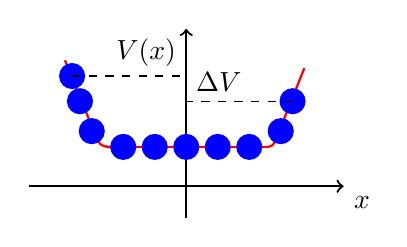
\begin{tikzpicture}
		\coordinate (a) at (-1,0.5);
		\coordinate (b) at (1,0.5);
		\coordinate (a1) at (-1.5,1.5);
		\coordinate (b1) at (1.5,1.5);
		\draw[thick,->] (-2,0) -- (2,0)node[anchor= north west] {\(x\)} ;
		\draw[thick,->] (0,-0.4) -- (0,2)node[anchor= north east]{\(V(x)\)};
		\draw [thick, red,rounded corners=0.6mm] (-1.54,1.6) -- (a1) --(-1.1,0.52)-- (a)  --  (b) -- (1.1,0.5) --(b1);
		 \node[circle,minimum size =0.07cm,
		fill=blue] (c) at (0,0.5){};
		\node[circle,minimum size =0.07cm,
		fill=blue] (c) at (0.4,0.5){};
		\node[circle,minimum size =0.07cm,
		fill=blue] (c) at (0.8,0.5){};
		\node[circle,minimum size =0.07cm,
		fill=blue] (c) at (1.2,0.7){};
		\node[circle,minimum size =0.07cm,
		fill=blue] (c) at (1.35,1.08){};
		\node[circle,minimum size =0.07cm,
		fill=blue] (c) at (-0.4,0.5){};
		\node[circle,minimum size =0.07cm,
		fill=blue] (c) at (-0.8,0.5){};
		\node[circle,minimum size =0.07cm,
		fill=blue] (c) at (-1.2,0.7){};
		\node[circle,minimum size =0.07cm,
		fill=blue] (c) at (-1.35,1.08){};
		\node[circle,minimum size =0.07cm,
		fill=blue] (c) at (-1.45,1.4){};
		\draw[dashed] (-1.45,1.4)node[anchor= south east] {} -- (0,1.4);
		\draw[dashed] (1.35,1.08)node[anchor= south west] {} -- (0,1.08) node[anchor= south west]  {\(\Delta V\)};
	\end{tikzpicture}
	\caption{\centering Difference in Fermi energy at both sides Edge's potential \(V(x)\)}
	\label{V without fill}
\end{figure}
\quad Considering the system in with the edge characterized by the potential \(V(x)\), shown in Fig. \ref{V without fill}. The group velocity can be obtained as
\begin{equation*}
	v_{k_y} = \frac{1}{\hbar}\pdv{E_{k_y}}{k_y}
\end{equation*}
\quad Using results from eq. \eqref{E general with V} to get
\begin{equation}
	v_{k_y} = -\frac{1}{eB}\pdv{V}{x}
\end{equation}
\quad From this, we can calculate the current of system:
\begin{align}
	I_y =&-\frac{e}{2\pi}\int v_{k_y}dk_y = \frac{e}{2\pi B}\int \pdv{V}{x} dx \frac{eB}{\hbar}\nonumber
	\\=& \frac{e^2}{2\pi \hbar} \Delta V
	= \frac{e^2}{2\pi \hbar} U_{x}
\end{align}
\quad The ratio give us the Hall conductivity of exact one Landau level
\begin{equation}
	\sigma_{yx} = \frac{I_y}{U_x} = \frac{e^2}{2\pi \hbar}
\end{equation}
As we can see that the overall \(I_y\) will be depended only from the difference between two side of the system's potential. No matter what kind of function of \(V(x)\) is, if the Fermi level are higher than the middle of the function and \(V(x)\) is smooth in that range, then the macro phenomenon will affected by the edge of the system, called \textit{edge mode}.
\subsection{Role of Disorder}
\quad The other aspect that weren't covered is the role of disorder in the existence of the plateaus. We will showing that, the impurity play a key roles in the existence of the continuous plateaus. \\\null\quad Quantizating the center of mass \((X,Y)\) from \eqref{r classical}
\begin{align}\label{X,Y or. def}
	\begin{split}
x_0 \to X(t) &= x + \frac{1}{\omega_B} \dot{y} = x+ \frac{\pi_y}{m \omega_B}\\
y_0 \to Y(t) &= y- \frac{\pi_x}{m \omega_B},
	\end{split}
\end{align}
\quad which some properties \footnote{\(\comm{X}{Y} = \frac{i\hbar}{m\omega_B} = \frac{i\hbar}{eB} = il_B^2\)}\footnote{\(\comm{X}{H} = \comm{x + \frac{\pi_y}{m\omega_B}}{H} = 0 \leftarrow \comm{\pi_x}{\pi_y} = iq\hbar B\)}, which sometime can be called as the Heisenberg uncertainty of the oscillation. Putting it in the equation of motions:
\begin{equation}\label{center of mass}
	\begin{split}
		i\hbar \dv{X}{t} =& \comm{X}{H + V} = \comm{X}{H} + \comm{X}{V} = [X,V]\nonumber\\
		=&[X,Y] \pdv{V}{Y}= i l_B^2 \pdv{V}{Y}\\
		i\hbar \pdv{Y}{t} =& -il_B^2 \pdv{V}{X}.
	\end{split}
\end{equation}
\quad These equations showing that the center of the circle will drift along the equipotentials.\\\null\quad
\begin{figure}[!h]
\centering
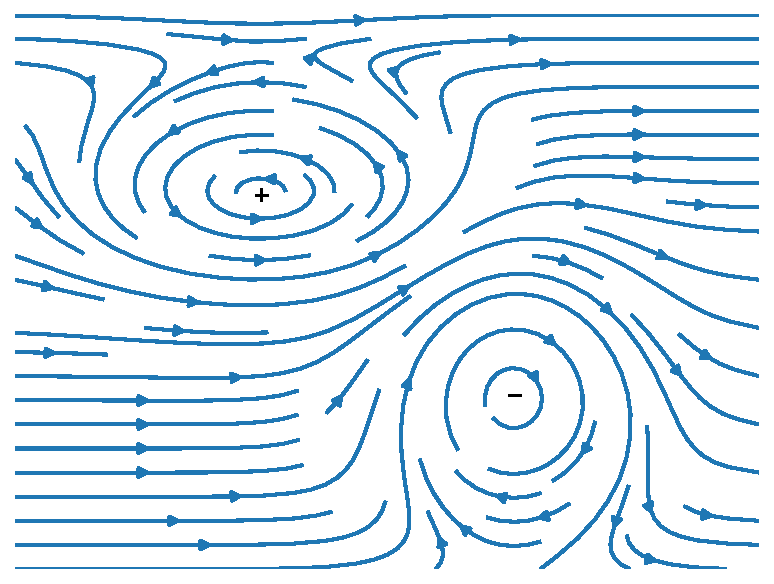
\includegraphics[width = 0.9\linewidth]{images/Disorder.pdf}
\caption{The movement of particles around the minima and maxima}
\label{Disorder}
\end{figure}\\\null
\quad The sample that we measure on, will never be a perfect one. It will have some dust on the surface or have some improper cell that break the total symmetry. Overall, the \textit{impurity} can be characterized as random peaks of the potential on the surface. Using the set of equations Eq. \eqref{center of mass}, we plot in Fig. \ref{Disorder} the flow of the center of the electron's circle when it flow through the sample.\\\null
\quad The particle that can move freely through the sample can be illustrated as the line that can move from the left to the right continuously. The one that being trapped around the maxima (\(+\)) and minima (\(-\)).\\\null
\quad These trapped particles will have the results in the spread out of the density of states (DOS), results in both edges of the peak about the Landau energy level as shown in Fig. \label{Disorder peak}.
\begin{figure}[!h]
\centering
\subfigure[{\small Without disorder}]{\scalebox{0.8}{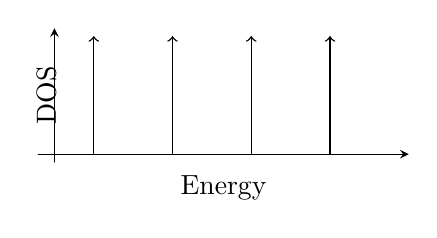
\begin{tikzpicture}[line cap=round,line join=round]
\definecolor{grannysmithapple}{rgb}{0.66, 0.89, 0.63}
\definecolor{unitednationsblue}{rgb}{0.36, 0.57, 0.9}
\begin{axis}[ticks=none,
x=1cm,y=1cm,
axis lines=middle,
xmin=-0.2052410812264766,
xmax=4.5,ymin=-0.1,x label style={at={(axis description cs:0.5,-0.03)},anchor=north}, y label style={at={(axis description cs:-0.03,0.5)},rotate=90},
ymax=1.6,xlabel=Energy,ylabel=DOS]
\draw [->,line width=0.5pt] (0.5,0) -- (0.5,1.5);
\draw [->,line width=0.5pt] (1.5,0) -- (1.5,1.5);
\draw [->,line width=0.5pt] (2.5,0) -- (2.5,1.5);
\draw [->,line width=0.5pt] (3.5,0) -- (3.5,1.5);
\end{axis}
\end{tikzpicture}}}\qquad
\subfigure[{\small with disorder}]{\scalebox{0.8}{\begin{tikzpicture}[line cap=round,line join=round]
		\begin{axis}[every axis plot post/.append style={
				mark=none,domain=-2:4,samples=100,smooth},ticks=none,
			x=1cm,y=1cm,
			axis lines=middle,
			xmin=-0.2052410812264766,
			xmax=4.5,
			ymin=-0.1,x label style={at={(axis description cs:0.5,-0.03)},anchor=north}, y label style={at={(axis description cs:-0.03,0.5)},rotate=90},
			ymax=1.6,xlabel=Energy,ylabel=DOS]
			
\addplot[color=black] {gauss(0.5,0.1)};
%\addplot {gauss(0.5,0.05)};
\addplot[color=black] {gauss(1.5,0.1)};
\addplot[color=black] {gauss(2.5,0.1)};
\addplot[color=black] {gauss(3.5,0.1)};
\addplot[color=black] {gauss(4.5,0.1)};

	\end{axis}
\end{tikzpicture}}}
\caption{The energy spectrum for without disorder (a) and with it (b).}
\end{figure}
\quad Not only that, the disorder also play an important role in the existence of the plateau in the spectrum. As shown in \eqref{degen ky}, the number of particle in a Landau level depend proportional to the magnetic field flux \(\Phi = B L_x L_y\). If in the initial, we fill the system up to \(n\)-th Landau level, and decrease the magnetic field \(B\). Now, each Landau level can accommodate less particles,
\begin{figure}[!ht]
	\begin{tikzpicture}[line cap=round,line join=round]
		\begin{axis}[every axis plot post/.append style={mark=none,domain=-2:4,samples=100,smooth},ticks=none,
			x=1cm,y=1cm,
			axis lines=middle,
			xmin=-0.2052410812264766,
			xmax=4.5,
			ymin=-0.1,x label style={at={(axis description cs:0.5,-0.03)},anchor=north}, y label style={at={(axis description cs:-0.03,0.5)},rotate=90},
			ymax=1.6,xlabel=Energy,ylabel=DOS]
			
			\addplot[color=black] {gauss(0.5,0.1)};
			%\addplot {gauss(0.5,0.05)};
			\addplot[color=black] {gauss(1.5,0.1)};
			\addplot[color=black] {gauss(2.5,0.1)};
			\addplot[color=black] {gauss(3.5,0.1)};
			\addplot[color=black] {gauss(4.5,0.1)};
			
		\end{axis}
	\end{tikzpicture}
\end{figure}
%	\section{Tables}\label{sec5}
%	
%	Tables can be inserted via the normal table and tabular environment. To put
%	footnotes inside tables one has to Lorem ipsum dolor sit amet, consectetur adipiscing elit, sed do eiusmod tempor incididunt ut labore et dolore magna aliqua. Ut enim ad minim veniam, quis nostrud exercitation ullamco laboris nisi ut aliquip ex ea commodo consequat. Duis aute irure dolor in reprehenderit in voluptate velit esse cillum dolore eu fugiat nulla pariatur. Excepteur sint occaecat cupidatat non proident, sunt in culpa qui officia deserunt mollit anim id est laborum. use the additional ``tablenotes" environment
%	enclosing the tabular environment. The footnote appears just below the table
%	itself (refer Tables~\ref{tab1} and \ref{tab2}).
%	
%	
%	\begin{verbatim}
%		\begin{table}[t]
%			\begin{center}
%				\begin{minipage}{<width>}
%					\caption{<table-caption>\label{<table-label>}}%
%					\begin{tabular}{@{}llll@{}}
%						\toprule
%						column 1 & column 2 & column 3 & column 4\\
%						\midrule
%						row 1 & data 1 & data 2          & data 3 \\
%						row 2 & data 4 & data 5$^{1}$ & data 6 \\
%						row 3 & data 7 & data 8      & data 9$^{2}$\\
%						\botrule
%					\end{tabular}
%					\begin{tablenotes}%
%						\item Source: Example for source.
%						\item[$^{1}$] Example for a 1st table footnote.
%						\item[$^{2}$] Example for a 2nd table footnote.
%					\end{tablenotes}
%				\end{minipage}
%			\end{center}
%		\end{table}
%	\end{verbatim}
%	
%	
%	Lengthy tables which do not fit within textwidth should be set as rotated tables. For this, we need to use \verb+\begin{sidewaystable}...+ \verb+\end{sidewaystable}+ instead of\break \verb+\begin{table}...+ \verb+\end{table}+ environment.
%	
%	
%	\begin{table}[!t]
%		\caption{Caption text\label{tab1}}%
%		\begin{tabular*}{\columnwidth}{@{\extracolsep\fill}llll@{\extracolsep\fill}}
%			\toprule
%			column 1 & column 2  & column 3 & column 4\\
%			\midrule
%			row 1    & data 1   & data 2  & data 3  \\
%			row 2    & data 4   & data 5$^{1}$  & data 6  \\
%			row 3    & data 7   & data 8  & data 9$^{2}$  \\
%			\botrule
%		\end{tabular*}
%		\begin{tablenotes}%
%			\item Source: This is an example of table footnote this is an example of table footnote this is an example of table footnote this is an example of~table footnote this is an example of table footnote
%			\item[$^{1}$] Example for a first table footnote.
%			\item[$^{2}$] Example for a second table footnote.
%		\end{tablenotes}
%	\end{table}
%	
%	\begin{table*}[t]
%		\caption{Example of a lengthy table which is set to full textwidth.\label{tab2}}
%		\tabcolsep=0pt%%
%		\begin{tabular*}{\textwidth}{@{\extracolsep{\fill}}lcccccc@{\extracolsep{\fill}}}
%			\toprule%
%			& \multicolumn{3}{@{}c@{}}{Element 1$^{1}$} & \multicolumn{3}{@{}c@{}}{Element 2$^{2}$} \\
%			\cline{2-4}\cline{5-7}%
%			Project & Energy & $\sigma_{calc}$ & $\sigma_{expt}$ & Energy & $\sigma_{calc}$ & $\sigma_{expt}$ \\
%			\midrule
%			Element 3  & 990 A & 1168 & $1547\pm12$ & 780 A & 1166 & $1239\pm100$\\
%			Element 4  & 500 A & 961  & $922\pm10$  & 900 A & 1268 & $1092\pm40$\\
%			\botrule
%		\end{tabular*}
%		\begin{tablenotes}%
%			\item Note: This is an example of table footnote this is an example of table footnote this is an example of table footnote this is an example of~table footnote this is an example of table footnote
%			\item[$^{1}$] Example for a first table footnote.
%			\item[$^{2}$] Example for a second table footnote.\vspace*{6pt}
%		\end{tablenotes}
%	\end{table*}
%	
%	\begin{sidewaystable}%[!p]
%		\caption{Tables which are too long to fit, should be written using the ``sidewaystable" environment as shown here\label{tab3}}
%		\tabcolsep=0pt%
%		\begin{tabular*}{\textwidth}{@{\extracolsep{\fill}}lcccccc@{\extracolsep{\fill}}}
%			\toprule%
%			& \multicolumn{3}{@{}c@{}}{Element 1$^{1}$}& \multicolumn{3}{@{}c@{}}{Element$^{2}$} \\
%			\cline{2-4}\cline{5-7}%
%			Projectile & Energy     & $\sigma_{calc}$ & $\sigma_{expt}$ & Energy & $\sigma_{calc}$ & $\sigma_{expt}$ \\
%			\midrule
%			Element 3 & 990 A & 1168 & $1547\pm12$ & 780 A & 1166 & $1239\pm100$ \\
%			Element 4 & 500 A & 961  & $922\pm10$  & 900 A & 1268 & $1092\pm40$ \\
%			\botrule
%		\end{tabular*}
%		\begin{tablenotes}%
%			\item Note: This is an example of a table footnote this is an example of a table footnote this is an example of a table footnote this is an example of a table footnote this is an example of a table footnote
%			\item[$^{1}$] This is an example of a table footnote
%		\end{tablenotes}
%	\end{sidewaystable}
%	
%	
%	\section{Figures}\label{sec6}
%	
%	As per display \LaTeX\ standards one has to use eps images for \verb+latex+ compilation and \verb+pdf/jpg/png+ images for
%	\verb+pdflatex+ compilation. This is one of the major differences between \verb+latex+
%	and \verb+pdflatex+. The images should be single-page documents. The command for inserting images
%	for \verb+latex+ and \verb+pdflatex+ can be generalized. The package used to insert images in \verb+latex/pdflatex+ is the
%	graphicx package. Figures can be inserted via the normal figure environment as shown in the below example:
%	
%	
%	\begin{figure}[!t]%
%		\centering
%		{\color{black!20}\rule{213pt}{37pt}}
%		\caption{This is a widefig. This is an example of a long caption this is an example of a long caption  this is an example of a long caption this is an example of a long caption}\label{fig1}
%	\end{figure}
%	
%	\begin{figure*}[!t]%
%		\centering
%		{\color{black!20}\rule{438pt}{74pt}}
%		\caption{This is a widefig. This is an example of a long caption this is an example of a long caption  this is an example of a long caption this is an example of a long caption}\label{fig2}
%	\end{figure*}
%	
%	
%	\begin{verbatim}
%		\begin{figure}[t]
%			\centering\includegraphics{<eps-file>}
%			\caption{<figure-caption>}
%			\label{<figure-label>}
%		\end{figure}
%	\end{verbatim}
%	
%	Test text here.
%	
%	For sample purposes, we have included the width of images in the
%	optional argument of \verb+\includegraphics+ tag. Please ignore this.
%	Lengthy figures which do not fit within textwidth should be set in rotated mode. For rotated figures, we need to use \verb+\begin{sidewaysfigure}+ \verb+...+ \verb+\end{sidewaysfigure}+ instead of the \verb+\begin{figure}+ \verb+...+ \verb+\end{figure}+ environment.
%	
%	\begin{sidewaysfigure}%
%		\centering
%		{\color{black!20}\rule{610pt}{102pt}}
%		\caption{This is an example for a sideways figure. This is an example of a long caption this is an example of a long caption  this is an example of a long caption this is an example of a long caption}\label{fig3}
%	\end{sidewaysfigure}
%	
%	
%	
%	\section{Algorithms, Program codes and Listings}\label{sec7}
%	
%	Packages \verb+algorithm+, \verb+algorithmicx+ and \verb+algpseudocode+ are used for setting algorithms in latex.
%	For this, one has to use the below format:
%	
%	
%	\begin{verbatim}
%		\begin{algorithm}
%			\caption{<alg-caption>}\label{<alg-label>}
%			\begin{algorithmic}[1]
%				. . .
%			\end{algorithmic}
%		\end{algorithm}
%	\end{verbatim}
%	
%	
%	You may need to refer to the above-listed package documentations for more details before setting an \verb+algorithm+ environment.
%	To set program codes, one has to use the \verb+program+ package. We need to use the \verb+\begin{program}+ \verb+...+
%		\verb+\end{program}+ environment to set program codes.
%	
%	\begin{algorithm}[!t]
%		\caption{Calculate $y = x^n$}\label{algo1}
%		\begin{algorithmic}[1]
%			\Require $n \geq 0 \vee x \neq 0$
%			\Ensure $y = x^n$
%			\State $y \Leftarrow 1$
%			\If{$n < 0$}
%			\State $X \Leftarrow 1 / x$
%			\State $N \Leftarrow -n$
%			\Else
%			\State $X \Leftarrow x$
%			\State $N \Leftarrow n$
%			\EndIf
%			\While{$N \neq 0$}
%			\If{$N$ is even}
%			\State $X \Leftarrow X \times X$
%			\State $N \Leftarrow N / 2$
%			\Else[$N$ is odd]
%			\State $y \Leftarrow y \times X$
%			\State $N \Leftarrow N - 1$
%			\EndIf
%			\EndWhile
%		\end{algorithmic}
%	\end{algorithm}
%	
%	Similarly, for \verb+listings+, one has to use the \verb+listings+ package. The \verb+\begin{lstlisting}+ \verb+...+ \verb+\end{lstlisting}+ environment is used to set environments similar to the \verb+verbatim+ environment. Refer to the \verb+lstlisting+ package documentation for more details on this.
%	
%	
%	\begin{minipage}{\hsize}%
%		\lstset{language=Pascal}% Set your language (you can change the language for each code-block optionally)
%		\begin{lstlisting}[frame=single,framexleftmargin=-1pt,framexrightmargin=-17pt,framesep=12pt,linewidth=0.98\textwidth]
%			for i:=maxint to 0 do
%			begin
%			{ do nothing }
%			end;
%			Write('Case insensitive ');
%			Write('Pascal keywords.');
%		\end{lstlisting}
%	\end{minipage}
%	
%	

	
%	\begin{unlist}
%		\item Sample unnumberd list text. Sample unnumberd list text. Sample unnumberd list text. Sample unnumberd list text. Sample unnumberd list text.
%		
%		\item Sample unnumberd list text. Sample unnumberd list text. Sample unnumberd list text.
%		
%		\item sample unnumberd list text. Sample unnumberd list text. Sample unnumberd list text. Sample unnumberd list text. Sample unnumberd list text. Sample unnumberd list text. Sample unnumberd list text.
%	\end{unlist}
	
\section{Fractional Hall Effect}
	
%	\medskip
%	\noindent\begin{tabular}{|l|p{13pc}|}
%		\hline
%		\verb+thmstyleone+ & Numbered, theorem head in bold font and theorem text in italic style \\\hline
%		\verb+thmstyletwo+ & Numbered, theorem head in roman font and theorem text in italic style \\\hline
%		\verb+thmstylethree+ & Numbered, theorem head in bold font and theorem text in roman style \\\hline
%	\end{tabular}
	
	
%	\begin{theorem}[Theorem subhead]\label{thm1}
%		Example theorem text. Example theorem text. Example theorem text. Example theorem text. Example theorem text.
%		Example theorem text. Example theorem text. Example theorem text. Example theorem text. Example theorem text.
%		Example theorem text.
%	\end{theorem}
	
	
%	\begin{proposition}
%		Example proposition text. Example proposition text. Example proposition text. Example proposition text. Example proposition text.
%		Example proposition text. Example proposition text. Example proposition text. Example proposition text. Example proposition text.
%	\end{proposition}
	
	
%	\begin{example}
%		Phasellus adipiscing semper elit. Proin fermentum massa
%		ac quam. Sed diam turpis, molestie vitae, placerat a, molestie nec, leo. Maecenas lacinia. Nam ipsum ligula, eleifend
%		at, accumsan nec, suscipit a, ipsum. Morbi blandit ligula feugiat magna. Nunc eleifend consequat lorem.
%	\end{example}
	
	
%	\begin{remark}
%		Phasellus adipiscing semper elit. Proin fermentum massa
%		ac quam. Sed diam turpis, molestie vitae, placerat a, molestie nec, leo. Maecenas lacinia. Nam ipsum ligula, eleifend
%		at, accumsan nec, suscipit a, ipsum. Morbi blandit ligula feugiat magna. Nunc eleifend consequat lorem.
%	\end{remark}
	
	
%	\begin{definition}[Definition sub head]
%		Example definition text. Example definition text. Example definition text. Example definition text. Example definition text. Example definition text. Example definition text. Example definition text.
%	\end{definition}
	
	
	
	\noindent
%	\begin{quote}
%		Quoted text example. Aliquam porttitor quam a lacus. Praesent vel arcu ut tortor cursus volutpat. In vitae pede quis diam bibendum placerat. Fusce elementum
%		convallis neque. Sed dolor orci, scelerisque ac, dapibus nec, ultricies ut, mi. Duis nec dui quis leo sagittis commodo.
%	\end{quote}
	
	\section{Conclusion}
	
	Some Conclusions here.
	
	%%%%%%%%%%%%%%
	
	\begin{appendices}	
	\section{Particle in Magnetic field}\label{particle in field}
\subsection{Cyclotron Oscillation}\label{Cyclotron}
\quad Considering an electron moves in a magnetic field perpendicular to the moving plane, the equation of motion for the particle charge -\(e\) and mass \(m\) is
\begin{equation}\label{Newton only B}
	m\dv{\textbf{v}}{t} = -e\textbf{v}\cross \textbf{B}
\end{equation}
\quad Solution for this equation is the oscillation of the electron around a circle:
\begin{equation}
	\textbf{r}(t) :
\begin{cases}\label{r classical}
	x(t)&= x_0 - R\sin(\omega_B t +\phi)\\
	y(t)&= y_0 + R\cos(\omega_B t +\phi)
\end{cases},
\end{equation}
\quad All these parameters are arbitrary, except the frequency \(\omega_B\), which is called cyclotron frequency:
\begin{equation}\label{cyclotron def}
	\omega_B = \frac{eB}{m},
\end{equation}
which clearly depend proportional to magnetic field \(B\).
\subsection{Drude Model}\label{Drude model appendix}
\quad Putting the system into the external electric field \(\textbf{E}\) along Ox and keep the magnetic field \(\textbf{B}\) perpendicular the Oxy plane, the equation of motion become:
\begin{equation}
	m \dv{\textbf{v}}{t} = -e\textbf{E} -e \textbf{v}\cross\textbf{B} - \frac{m \textbf{v}}{\tau},
\end{equation}
\quad in which the last term corresponding to the scattering of the electron characterized by the parameter \(\tau\), called scattering time. If the system archive the equilibrium, then
\begin{equation}\label{Hall origin.}
	\textbf{E} = \textbf{v}\cross\textbf{B} - \frac{m\textbf{v}}{\tau e}.
\end{equation}
\quad Substituting the current density \(J\) into \eqref{Hall origin.} through
\begin{equation}\label{J def.}
	\textbf{J} = -n e \textbf{v},
\end{equation}
to have Ohm's law in the matrix form:
\begin{equation}\label{Ohm def.}
\begin{pmatrix}
	1 & \omega_B \tau\\
	-\omega_B\tau & 1
\end{pmatrix}
\begin{pmatrix}
J_x \\J_y
\end{pmatrix} =\frac{e^2 n \tau}{m} \begin{pmatrix}
E_x \\ E_y
	\end{pmatrix},
\end{equation}
or in the inverse form
\begin{equation}\label{Ohm Inv.}
	\textbf{J} = \sigma \textbf{E}.
\end{equation}
\quad In which, the \(\sigma\) was called the \textit{conductivity tensor}. Without the present of the magnetic field \(\textbf{B}\), \eqref{Ohm Inv.} reduce to the DC conductivity form:
$$\textbf{J} = \sigma_{DC} \textbf{E}\quad  \text{ with } \quad \sigma_{DC} = \frac{ne^2 \tau}{m},$$
\quad For general case, we derive explicitly from \eqref{Ohm def.}:
\begin{equation}
	\sigma = \frac{\sigma_{DC}}{1 + \omega_B^2 \tau^2} \begin{pmatrix}
		1 & -  \omega_B\tau\\
		\omega_B \tau & 1
	\end{pmatrix}
\end{equation}
\section{Landau Levels}\label{Landau level}
\quad Considering 2-D system confined within Oxy plane with the magnetic field being placed perpendicular to the system.
\subsection{Landau Gauge}
\quad Fixing the gauge by choosing the Landau gauge (\(\textbf{A} = (0,Bx,0), \phi = 0\), which is vector and scalar potential of the electromagnetic field, respectively), the Hamiltonian of the system reads:
\begin{align}
	H &= \frac{(\textbf{p}+e\textbf{A})^2}{2m}\nonumber\\
	\label{Landau H}
	&= \frac{p_x^2}{2m} + \frac{(p_y+eBx)^2}{2m} +\frac{p_z^2}{2m}.
\end{align}
\quad In this convention, there is no \(y, z\) in this Hamiltonian. Therefore, we have an Ansatz:
\begin{equation}\label{Landau ansatz}
	\psi(x,y,z) = e^{i(k_yy + k_z z)}\psi_x(x).
\end{equation}
\quad Substituting \eqref{Landau ansatz} and \eqref{Landau H} into Schrödinger equation to have\footnote{In this case , we note that \([H,y] = [H,z] = 0\), leave the \(p_y\) as a constant}:
\begin{equation}\label{Landau ansatz 1}
	\bigg(\frac{p_x^2}{2m} + \frac{(\hbar k_y + eBx)^2}{2m} + \frac{\hbar^2 k_z^2}{2m}\bigg)\psi_x(x) = E_{k_y,k_z}\psi_x(x).
\end{equation}
\quad Excluding the free or extreme confined part of \(k_z\) depend on the system, \eqref{Landau ansatz 1} leaves us with:
\begin{equation}\label{Landau HO}
	\bigg(\frac{p_x^2}{2m} + \frac{m\omega_B^2 }{2}\bigg(x+\frac{\hbar k_y}{eB}\bigg)^2\bigg)\psi_{x}(x) = E_{k_y} \psi_{x}(x).
\end{equation}
\quad Using the same convention for the harmonic oscillator, we introduce the ladder operators:
\begin{align}
	\hat{x}-k_y l_B^2 &= \sqrt{\frac{\hbar}{2m \omega_B}} \big(a^\dagger + a\big),\quad l_B^2 = \frac{\hbar}{eB},\\
	\hat{p} &=i\sqrt{\frac{\hbar m\omega_B}{2}}\big(a^\dagger - a\big).
\end{align}
\quad Which allow us to rewrite the Hamiltonian in term of these ladder operators:
\begin{equation}\label{Landau Level Hamiltonian}
	H = \hbar\omega_B \bigg(\frac{1}{2} + a^\dagger a\bigg) = \hbar\omega_B \bigg(\frac{1}{2} + n_x\bigg)
\end{equation}
\quad From here, we clearly seeing that the eigenvalue have discrete value of \(\hbar \omega_B\), which in turn corresponding to the \(k_y\).\\\null
\quad Overall, the wave function now depend on two quantum numbers \(n \in \mathbb{N}\) and \(k_y \in \mathbb{R}\):
\begin{equation*}
	\psi_{n,k_y} \sim e^{ik_y y} H_n(x + kl_B^2) e^{-\frac{(x+ k l_B)^2}{l_B^2}}
\end{equation*}
\quad Considering the particle in the box with the length of Oy is \(L_y\), the boundary condition give us:
\begin{equation}\label{k_y BC}
	k_y = \frac{N2\pi}{L_y},\quad N \in \mathbb{Z},
\end{equation}
give us a very large number of degeneracy states. Applying the boundary condition x direction, the particle have to stay inside the box:
\begin{equation*}
	0\leq x \leq L_x
\end{equation*}
At each degeneracy \(k_y\), the particle will oscillate about the point \(x = -k_y l_B^2\). Therefore, these is limit for \(k\):
\begin{equation*}
	-\frac{L_x}{l_B^2}\leq k_y \leq 0.
\end{equation*}
Give us the total number of state inside the box for one filled Landau level:
\begin{equation} \label{degen ky}
	\mathrm{N} = \frac{L_y}{2\pi}\int_{-\frac{L_x}{l_B^2}}^0 dk = \frac{L_y L_x}{2\pi l_B^2} = \frac{L_x L_y eB}{2\pi \hbar}.
\end{equation}
\quad Since there is no difference in the density of states for the other level \(n\), the density of states spectrum can be seen as multiple poles, called 'Dirac comb' (not Dirac cone, sound a like and have a little connection between both of it). A little remind about the density of state for an 2-D free electron gas is it a reverse Heavyside function at \(E = E_F\), when applying the magnetic field, it concentrate into the pole with insane number in a small width that can be seen as Dirac delta function.
\begin{figure}[!ht]
\centering
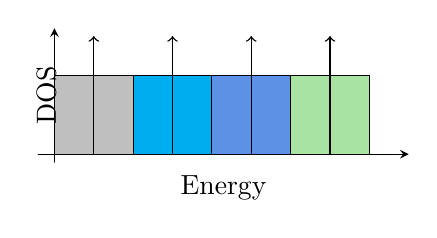
\begin{tikzpicture}[line cap=round,line join=round]
	\definecolor{grannysmithapple}{rgb}{0.66, 0.89, 0.63}
	\definecolor{unitednationsblue}{rgb}{0.36, 0.57, 0.9}
	\begin{axis}[ticks=none,
		x=1cm,y=1cm,
		axis lines=middle,
		xmin=-0.2052410812264766,
		xmax=4.5,
		ymin=-0.1,x label style={at={(axis description cs:0.5,-0.03)},anchor=north}, y label style={at={(axis description cs:-0.03,0.5)},rotate=90},
		ymax=1.6,xlabel=Energy,ylabel=DOS]
		\filldraw[draw=black,fill=lightgray] (0,0) rectangle (1,1);
		\filldraw[draw=black,fill=cyan] (1,0) rectangle (2,1);
		\filldraw[draw=black,fill=unitednationsblue] (2,0) rectangle (3,1);
		\filldraw[draw=black,fill=grannysmithapple] (3,0) rectangle (4,1);
		\draw [->,line width=0.5pt] (0.5,0) -- (0.5,1.5);
		\draw [->,line width=0.5pt] (1.5,0) -- (1.5,1.5);
		\draw [->,line width=0.5pt] (2.5,0) -- (2.5,1.5);
		\draw [->,line width=0.5pt] (3.5,0) -- (3.5,1.5);
		\draw [line width=0.5pt] (4,1)-- (4,0);
	\end{axis}
\end{tikzpicture}
\vspace{-1.3cm}
\caption{Dirac comb with constant DOS of 2D Fermi gas in background}
\end{figure}\\\null
\quad But in this case, clearly seeing that not only the symmetry in translation along \(x\) axis have been broke: \([x,H] \neq 0\), also with the rotation symmetry about the z axis also has been broke:
\begin{equation}
	[\hat{H}, \hat{L}_z] = [\hat{H}, x \partial_y - y\partial_x] = - [H, y\partial_x] \neq 0
\end{equation}
\subsubsection{Including The Electric Field}
\quad If we including the electric field into the system along Ox, we have the Hamiltonian:
\begin{equation}
	H = \frac{(p_x^2 + (p_y-eBx)^2)}{2m} + eEx
\end{equation}
With a little manipulate, we have:
\begin{align}
	H =& \frac{p_x^2}{2m} + \frac{\hbar^2 k_y^2 - 2\hbar k_y eB x + (eBx)^2 + 2meEx}{2m}\nonumber\\
	=& \frac{p_x^2}{2m} + (eB)^2\frac{x^2 -2x(\hbar k_y /eB - mE/e^2B)}{2m} + \frac{\hbar^2 k_y^2}{2m}\nonumber\\
	\label{x shifted in em field}
	=& \frac{p_x^2}{2m} + \frac{e^2 B^2}{2m}\bigg(x- \frac{\hbar k_y}{eB} + \frac{mE}{eB^2}\bigg)^2\nonumber\\ &-eE\bigg(k_y l_B^2 + \frac{eE}{m \omega^2_B}\bigg) + \frac{m}{2}\frac{E^2}{B^2}
\end{align}
\begin{equation}\label{eigen energies in emf}
	E_{n,k}= \hbar \omega_B \bigg(n+\frac{1}{2}\bigg) - eE\bigg(kl_B^2 + \frac{eE}{m\omega_B^2}\bigg) + \frac{m}{2}\frac{E}{B}
\end{equation}
The eigenstates are the same but with an extra shift \(-\frac{mE}{e B^2}\).
\subsubsection{An Useful Note}
\quad A worthy more generalized note need to talk about for later use. Considering the Hamiltonian have the form:
\begin{equation*}
H = \frac{(p_x^2 + (p_y+eBx)^2)}{2m} + V(x)
\end{equation*}
\quad Expanding the potential \(V(x)\) by Taylos's series around some point \(x_0\), neglect the quadratic term to have:
\begin{equation*}
	H = \frac{(p_x^2 + (p_y+eBx)^2)}{2m} + V_0(x_0) + \pdv{V(x)}{x}\bigg|_{x=x_0} (x-x_0).
\end{equation*}
\quad Choosing the ground potential \(V_0 (x_0)\) and the origin of the reference frame to have
\begin{equation}
		H = \frac{(p_x^2 + (p_y-eBx)^2)}{2m} + \pdv{V(x)}{x}\bigg|_{x=x_0} x.
\end{equation}
\quad Doing the sane process as \eqref{x shifted in em field}, we arrive with the eigenenergies:
\begin{equation}\label{E general with V}
	E_{n,k,x}= \hbar \omega_B \bigg(n+\frac{1}{2}\bigg) - e\nabla_x V\bigg(kl_B^2 + \frac{e\nabla_x V}{m\omega_B^2}\bigg) + \frac{m}{2}\frac{\nabla_x V}{B}
\end{equation}
\quad The \(k_y\) and \(x\) have the relation for the shift of wave function: \(x= -kl_B^2 + \frac{m\nabla_x V}{eB^2}\).
\subsubsection{Symmetric Gauge}
\quad This lead us to an adaptation, choosing a symmetric gauge:
\begin{equation}\label{Symmetric Gauge}
	\textbf{A} = -\frac{1}{2} \textbf{r} \cross \textbf{B} = -\frac{y B}{2} \vec{i} + \frac{x B}{2} \vec{j}.
\end{equation}
\quad This convention broke translation symmetry in both \(x\) and \(y\) directions. On another hand, it reserve the rotation symmetry about the z-axis:
$$[H,x \partial_y - y\partial_x] = 0$$
in which,
\begin{equation}
	H = \frac{(p_x - yeB/2)^2}{2m} + \frac{(p_y + xeB/2)^2}{2m}.
\end{equation}
\quad Due to this convention, the canonical momentum vector has to be defined:
 \begin{align}
     \bm{\pi} &= \textbf{p} - q\textbf{A}= \textbf{p} + e\textbf{A},\\\label{pi com.}
     \comm{\pi_x}{\pi_y} &= iq\hbar \bigg(\pdv{A_y}{x} - \pdv{A_x}{y}\bigg) = iq\hbar B\\
 	 a&= \frac{1}{\sqrt{2\hbar B}} (\pi_x + i\pi_y),
 \end{align}
\quad In contract with the canonical  momentum \(\textbf{p}\), the mechanical momentum \(\bm{\pi}\) is the one represent the kinetic of the particle in the laboratory frame, therefore it is called "Kinetic momentum" sometime. Which give
\begin{align*}
	[a,a^\dagger] &= 1,\\
	H = \frac{1}{2} \bm{\pi}\cdot\bm{\pi} &= \hbar \omega_B (a^\dagger a +\frac{1}{2}).
\end{align*}
Defining another operator:
\begin{equation}
\bm{\tilde{\pi}} = \textbf{p} - e\textbf{A},
\end{equation}
this choice is \textbf{not} \textit{gauge invariant} (for more information, see appendix \ref{gauge invariance}). The commutator of the new operators obeys:
\begin{equation}
	[\bm{\tilde{\pi}}_x,\bm{\tilde{\pi}}_y] = ie\hbar B.
\end{equation}
\quad The commutator this new operators and the mechanical momentum:
\begin{equation}
	[\pi_x,\tilde{\pi}_x] = 2 i e\hbar \pdv{A_x}{x},\quad [\pi_y,\tilde{\pi}_y] = 2 i e\hbar \pdv{A_y}{y}
\end{equation}
\begin{equation}
\quad [\pi_x,\tilde{\pi}_y] = [\pi_y,\tilde{\pi}_x] = ie\hbar \left(\pdv{A_x}{y} + \pdv{A_y}{x}\right)
\end{equation}
\quad By the choice of symmetric gauge \ref{Symmetric Gauge}, all the commutators above vanish. Allow define new ladder operators:
\begin{equation}
	b = \frac{1}{\sqrt{2 e\hbar B}}(\tilde{\pi}_x + i \tilde{\pi}_y); \quad 	b^\dagger = \frac{1}{\sqrt{2 e\hbar B}}(\tilde{\pi}_x - i \tilde{\pi}_y)
\end{equation}
\quad These two operators obey
$$[b,b^\dagger] = 1$$
\quad From this, we can construct the wave function as the simple harmonic for two set of operator:
$$a \ket{0,0} = b\ket{0,0} = 0$$
$$\ket{n,m} \equiv  \frac{(a^\dagger)^n (b^\dagger)^m}{\sqrt{m!n!}} \ket{0,0}$$
\section{Berry Phase and Some Relations}
...
\subsection{Abelian Berry Phase and Berry Connection}
\quad Considering a generalize Hamiltonian, expressed in term of degree of freedoms \(x^\alpha\), in example: position or spins, and parameters \(\lambda^i\), in example, the spring constant in the harmonic oscillator problem.
$$H= H(x^\alpha, \lambda^i).$$
\quad Now, gently varying the parameter in respect to the time with an assuming that in the initial time, the system is in the eigenstate \(\ket{\psi}\): \(\ket{\psi} \to \ket{\psi(\lambda(t))}\). The parameter will be vary so gentle that the system can't be excited to another eigenstate, we don't talk about degeneracy, at least at this point.\\\null
\quad Finally, the parameter have to return to the same value as if when it start to move, making a closed trajectory in the parameter space. Since the starting point is the eigenstate, the final state have to be proportional to it initial state: \(\ket{\psi} \to e^{i\gamma}\ket{\psi}\). Neglect the evolution term in respect with the time \(exp(-iEt/\hbar)\), there is still another phase that contribution to the global phase, called \textit{Berry phase}.
\subsection{Calculate the Berry Phase}
\quad At time \(t\), the Hamiltonian have solution \(\ket{\psi(t)}\). Assuming that they can be expand in the basis \(\{\ket{n(t)}\}\) that satisfied the time-independence Schrödinger equation:
\begin{equation}
	H(t) \ket{n(t)} = E_n(t) \ket{n(t)}
\end{equation}
From Schrödinger equation,
\begin{align*}
	i\hbar \partial_t \ket{\psi(t)} &= H(t)  \ket{\psi(t)}\\
	i \hbar \sum_{n}\partial_t c_n(t) \ket{n(t)} &= \sum_{n}H(t) c_n(t)\ket{n(t)}\\
	i\hbar \sum_{n} \dot{c}_n(t) \ket{n(t)} + c_n(t) \dot{\ket{n(t)}} &= \sum_{n}c_n(t) E_n(t) \ket{n(t)}
\end{align*}
\quad Multiplying both sides with \(\bra{m(t)}\) and using the eigenstate orthogonal properties
\begin{align*}
	i\hbar \dot{c}_m(t) + i\hbar \sum_{n} c_n(t) \braket{m(t)}{\dot{n(t)}} &= c_m(t) E_m(t)\\
	\dot{c}_m (t) +  c_m(t) \bigg( \braket{m(t)}{\dot{m(t)}}+ i\frac{E_m(t)}{\hbar}\bigg) &= \sum_{n \neq m} c_n(t) \frac{\bra{m(t)} \dot{H} \ket{n(t)}}{E_m(t) - E_n(t)}
\end{align*}
\quad Using the assuming that \(\frac{\dot{H}}{E_m(t) - E_n(t)}\) too small and  \(E_m(t) - E_n(t) \neq 0\) with \(m \neq n\) to neglect this term, then
\begin{align}
	\dot{c}_m(t) &= -c_m(t) \bigg(i\frac{E_m(t)}{\hbar} + \braket{m(t)}{\dot{m(t)}}\bigg)\\
	\label{before include Berry connection}
	\Rightarrow c_m(t) &= c_m(0) e^{- \int_0^t(i\frac{E_m(t')}{\hbar} + \braket{m(t')}{\dot{m(t')}}) dt'}.
\end{align}
\quad In here, we define the \textit{Berry connection} (or Berry potential):
\begin{equation}\label{Berry con. def.}
	\mathcal{A}_i(\lambda) \equiv i\bra{n(t)} \pdv{ }{\lambda^i} \ket{n(t)}
\end{equation}
\quad Substituting into \eqref{before include Berry connection} to get
\begin{equation}
	c_m(t) = c_m(0) e^{-\int_0^t \frac{iE_m(t')}{\hbar}}e^{i\gamma},
\end{equation}
in which
$$\gamma = \oint_C \mathcal{A}_i d \lambda^i$$
\quad Instead of depend on the varying time, \textit{geometry phase} depend on the path of the parameter in the parameter space. The term
$$e^{i\oint_C \mathcal{A}_i d \lambda^i}$$
will be called \textit{Berry phase}.\\\null
\quad In the same spirit with the gauge transformation in electromagnetism, the physical information can be extract by calculating the \textit{Berry curvature} of the connection,
\begin{equation}
	\mathcal{F}_{ij}(\lambda) \equiv \pdv{\mathcal{A}_i}{\lambda^j} -\pdv{\mathcal{A}_j}{\lambda^i}.
\end{equation}
\quad Using Stokes's theorem for the \textit{Berry phase}
$$e^{i\gamma} = exp\bigg(-i \oint_C \mathcal{A}_i(\lambda) d\lambda^i\bigg) = exp\bigg(-i \int \mathcal{F}_{ij} dS^{ij}\bigg)$$
With the \(S_{ij}\) is the surface which being closed by contour \(C\)\footnote{An interesting example can be found in the Tong's lecture note}.
\subsection{Chern Number}
%\subsubsection{Kubo's Formula}
%\quad It worth to mention about an approach for further calculation, it's \textit{linear response}. Defining the Hamiltonian consist of two part:
%$$H = H_0 + V(t)\theta(t-t_0)$$
%in which \(H_0\) is the unperturbed multi-particle Hamiltonian, \(V(t)\) is the time-dependence perturbation part, \(\theta(t)\) is the Heaviside function.\\ \null
%\quad Assuming that we prepare the system in a state \(\ket{0}\) from the initial \(t \to -\infty\). The time-evolution of an time-dependence operator \(A(t)\) will be:
%\begin{equation}
%	\ev{A(t)} = \ev{A}_0 +\frac{i}{\hbar} \int_{-\infty}^{t}[V(t'),A(t)]dt'
%\end{equation}
%\quad In this case, the particles was placed in electric field with vector potential \(\textbf{A}\):
%\begin{equation}
%	H = H_0 + e\textbf{J}.\textbf{A}
%\end{equation}
\subsection{Aharonov-Bohm effect}
\quad In two-split experiment for electron, we place a solenoid in between two split and the screen (include graphic on Aharonov-Bohm effect). This solenoid will be put in some kind of "concrete", which will eliminate all magnetic field \(B\) outside of it's wall. According to the Stoke's theorem for a circle with radius \(r\) bigger than the wall:
\begin{equation}
	\Phi = \int \textbf{B} d\textbf{S} = \int_{in} (\nabla \times \textbf{A}) dS = \oint_C \textbf{A} dl
\end{equation}
\quad According to the gauge invariance, we can chose \(\textbf{A}\) freely. By choosing \(\textbf{A}\) that have angular symmetry, it will give us a specific magnetic flux that we will need later:
\begin{equation}\label{solenoid gauge}
	\Phi = A_{\phi} 2\pi r \Rightarrow A_{\phi} = \frac{\Phi}{2\pi r}
\end{equation}
\subsubsection{Long story short}
\quad The solenoid will stay somewhere between two split (not right in the middle, it will be too perfect) and near the split's wall so that the particle can not pass by the solenoid, it still effected by the potential vector \(\textbf{A}\) from that solenoid, causing phase difference for electron depend on whether they pass upper or below split. The results will be the shift in the spectrum on the screen. As we chance the \(\textbf{B}\) in the solenoid, \(\textbf{A}\) will also chance and causing the spectrum to chance (can be spread out, narrow in or moving left and right).
\subsubsection{Long story long}
\quad Put a particle into a box, the box will stay near some magnetic field \(\textbf{B}\) shielded. The box has to be small enough that the vector potential \(\textbf{A}\) is constant within the box. Hamiltonian of the particle will be:
\begin{equation}
	H = \frac{1}{2m} (\textbf{p} + e\textbf{A}(\textbf{X}))^2 + V(x-X),
\end{equation}
in which \(\textbf{X}\) is the center of the box. Choosing the gauge at the initial position so that \(\textbf{A}(\textbf{X}_0) = 0\). At the initial, the particle will stay in the ground state:
$$\psi_0(x-X_0).$$
\quad Slowly move the box to another position \(X\), the wave function will be:
$$\psi(x-X) = exp\bigg(-\frac{ie}{\hbar} \int_{\textbf{X}_0}^{\textbf{X}} \textbf{A}(\textbf{x}) d\textbf{x}\bigg) \psi(\textbf{x}-\textbf{X}_0)$$
\quad If the box move along a closed path \(C\), compare two wave function:
$$\psi(x-X_0) \to e^{i\gamma} \psi(\textbf{x} - \textbf{X}_0)=exp\bigg(-\frac{ie}{\hbar} \oint_C \textbf{A}(\textbf{x}) d\textbf{x}\bigg) \psi(\textbf{x}-\textbf{X}_0)$$
\quad Easily seeing from the generalize definition of \textit{Berry phase} the relation for magnetic field:
$$\bm{\mathcal{A}}(\textbf{X}) = \frac{e}{\hbar} \textbf{A}(\textbf{x}= \textbf{X})$$
\quad Generally, if a particle with charge \(q\) move around a region with magnetic flux \(\Phi\), it will pick up a Aharonov-Bohm phase:
\begin{equation} \label{AB phase}
	e^{i\frac{q}{\hbar} \Phi}
\end{equation}
\subsubsection{Spectral Flow}
Consider an electron move only in a circle around the localized solenoid. As we mentioned, the solenoid will be characterized by the magnetic flux \(\Phi\). It will be wise to choose the symmetry gauge \eqref{solenoid gauge} around the z-axis, the Hamiltonian of the system will have the form:
\begin{equation}
	H = \frac{1}{2m}(p_{\phi} - qA_\phi)^2=\frac{1}{2mr^2} \bigg(\frac{\hbar}{i} \partial_{\phi} - \frac{q\Phi_0}{2\pi}\bigg)^2.
\end{equation}
\quad The eigenvalues and eigenfunctions will be:
\begin{align}
	\psi_{n,r}(\phi) &= \frac{1}{\sqrt{2\pi r}}e^{in\phi},\\\label{eigenenergies of solenoid}
	E_n(\Phi) &= \frac{\hbar^2}{2mr^2} \bigg(n - \frac{q\Phi}{2\pi \hbar}\bigg)^2= \frac{\hbar^2}{2mr^2} \bigg(n + \frac{\Phi}{\Phi_0}\bigg)^2.
\end{align}
\quad In here, one again, we meet the \textit{quantum flux} \(\Phi_0 = \frac{h}{q} = \frac{2\pi \hbar}{e}\). From \eqref{eigenenergies of solenoid}, we seeing that in the case \(\forall \frac{\Phi}{\Phi_0} \in \mathrm{Z}\), the energy spectrum will be the same. Otherwise, as it should be since there is nothing constrains the external parameter \(\phi\) to be integer times of the quantum flux, the energy spectrum gets shifted.
\begin{equation*}
	\psi_n(\Phi) \xrightarrow{\Phi \to \Phi+\Phi_0} \psi_n(\Phi+\Phi_0) = \psi_{n+1} (\Phi)
\end{equation*}
\quad This is an interesting result, the particle never experience the magnetic field \(B\) inside the solenoid but still being affected by it vector potential \(\textbf{A}\) and results in the shift of energy spectrum. As we increase the magnetic flux by one time quantum flux \(\Phi \to \Phi + \Phi_0\), the energy of that particle will be shifted from \(E_n (\Phi) \to E_{n+1} (\Phi)\), increasing the quantum number \(n\) to \(n+1\).\\\null
\quad These results is an example of a brand of a wider situation called "spectral flow", whence under the chance of the external parameter, each individual state morphed into each others while spectrum chance from itself to itself.
\section{Remind Some Old Things}
\section{Gauge Invariance}\label{gauge invariance}
\quad In quantum mechanics, the field's gauge transform will have the form:
\begin{align*}
	\textbf{A} \to&\,\textbf{A}'= \textbf{A} + \nabla \Lambda\\
	\psi \to&\,\psi' = \psi e^{i\frac{q}{\hbar}\Lambda}
\end{align*}
\quad With any function \(\Lambda = \Lambda (x,y,z)\), this transformation work. But in contract, any \(\textbf{F}(x,y,z)\) which is not a gradient of any function that transform \(\textbf{A} \to \textbf{A}' =  \textbf{A} + \textbf{F}(x,y,z)\), will not work. For example, \(\Lambda = x^ny^m \,\forall n,m \in \mathbb{N}\), will work, but \(\textbf{F}(x,y,z) = (y,x,0)\) will not.\\
\null\quad The transformation of the wave function will cancel out the eigenvalue \(\pi\) of the observable, \(\bm{\pi} = \textbf{p} - q\textbf{A}\). Doing the transform
\begin{align*}
	\bm{\pi} \psi= \pi \psi \to \bm{\pi'} \psi'=& \bigg(\frac{\hbar}{i} \nabla - q\textbf{A} - q \textbf{A}\nabla \Lambda\bigg)\psi e^{i\Lambda/\hbar}\\
=& \bigg(\frac{\hbar}{i} \nabla \psi - q\textbf{A}\psi\bigg) e^{i\Lambda/\hbar} =\pi \psi e^{i\Lambda/\hbar}.
\end{align*}
\quad Vice versa, the opposite in sign is not, \(\tilde{\bm{\pi}} = \textbf{p} + q \textbf{A}\) in the transform give
\begin{align*}
	\tilde{\bm{\pi}} \psi = \tilde{\pi} \psi\to 	\tilde{\bm{\pi}}' \psi' =& \bigg(\frac{\hbar}{i} \nabla + q\textbf{A} + q \textbf{A}\nabla \Lambda\bigg)\psi e^{i\Lambda/\hbar}\\
	=& \bigg(\frac{\hbar}{i}\psi \nabla + q\textbf{A}\psi\bigg)e^{i\Lambda/\hbar} + 2 q \textbf{A}\psi\nabla \Lambda e^{i\Lambda/\hbar}\\
	=& \,\tilde{\pi}\psi e^{i\Lambda/\hbar} + 2 q \textbf{A}\psi\nabla \Lambda e^{i\Lambda/\hbar},
\end{align*}
\quad Definitely defend on the gauge choosing, or \textit{variance}.
	\end{appendices}
	\bibliographystyle{unsrtnat}
	\bibliography{reference}
\end{document}
